\problemname{Bakrum}

Trollkarlen Harry gillar att baka.
När han en dag hittade en trollformel för att transportera sig till ''bakrummen'' blev han fylld med lycka.
När han väl använde trollformeln transporerades han tyvärr inte till ett bageri, utan ett oändligt stort rutnät.
Varje ruta i rutnätet är antingen fri eller blockerad.
I rutnätet kan man vandra upp, ner, höger eller vänster till intilliggande rutor som inte är blockerade.
Efter att ha promenerat runt en bit märker han att vilka rutor som är blockerad följer ett periodiskt mönster.
Det finns ett $R \times C$ stort mönster som repeterar sig oändligt.
Se bilden nedan för exakt hur detta funkar.

\begin{figure}[h]
  \centering
  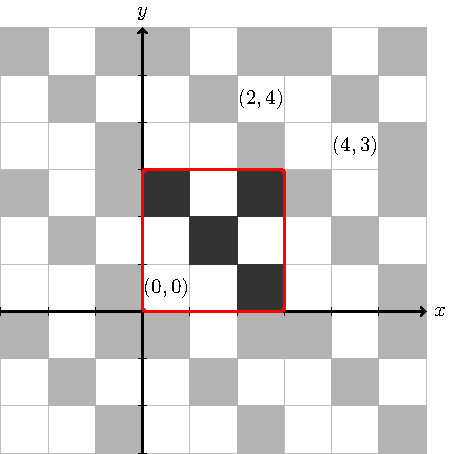
\includegraphics[width=0.3\textwidth]{sampleimage.pdf}
  \caption{Visualisering av exempelfall 2. Grundmönstret är markerat i rött och koordinaterna av den första frågan är ritade vid (2,4) och (4,3).
  Självfallet fortsätter rutnätet bortom det som ritats.}
\end{figure}

För att fly behöver han ta sig till en viss cell i rutnätet.
Hans teleportationsmagi är dock lite rostig, så han kommer därför ställa dig fem frågor på formen
''om jag teleporterar mig till rutan $(s_x, s_y)$, kan jag vandra till rutan $(g_x, g_y)$?''.

\section*{Indata}
Den första raden innehåller två heltal $R$ och $C$ ($1 \leq R,C \leq 5$), antalet rader och kolumner i rutnätet.

De följande $R$ radera innehåller vardera en sträng av längd $C$, som består av tecknen ''\verb|.|'' och ''\verb|#|''.
Det här är raderna i rutnätet. Tecknet ''\verb|#|'' betyder att det rutan är blockerad, och
''\verb|.|'' betyder att rutan är fri.

Därefter följer fem rader. Varje av dessa rader innehåller fyra heltal $s_x, s_y_, g_x, g_y$ ($0 \leq s_x, s_y, g_x, g_y \leq 10^{12}$),
koordinaterna på en fråga.

\section*{Utdata}
För varje fråga, skriv ut ''\texttt{Ja}'' om Harry kan vandra från ruta $(s_x, s_y)$ till ruta $(g_x, g_y)$, annars ''\texttt{Nej}''.

\section*{Poängsättning}
Din lösning kommer att testas på en mängd testfallsgrupper.
För att få poäng för en grupp så måste du klara alla testfall i gruppen.

\noindent
\begin{tabular}{| l | l | p{12cm} |}
  \hline
  \textbf{Grupp} & \textbf{Poäng} & \textbf{Gränser} \\ \hline
  $1$    & $20$  & $R, C \leq 2$ \\ \hline
  $2$    & $20$  & $s_x, s_y \leq 500$ \\ \hline
  $3$    & $20$  & $g_x, g_y \leq 10^5$ \\ \hline
  $4$    & $40$  & Inga ytterligare begränsningar. \\ \hline
\end{tabular}

